\pdfoutput=1
\documentclass[conference]{IEEEtran}
\IEEEoverridecommandlockouts
% The preceding line is only needed to identify funding in the first footnote. If that is unneeded, please comment it out.

\usepackage{times}
\usepackage{cite}
\usepackage{amsmath}
\usepackage{amssymb}
\usepackage{bm}
\usepackage{graphicx}
\usepackage{booktabs}
\usepackage{array}
\usepackage{url}
\usepackage{algorithm}
\usepackage{algpseudocode}
\usepackage[table]{xcolor}
\usepackage{xspace}

\newcolumntype{Y}{>{\raggedright\arraybackslash}X} % 左对齐+自动换行

\newcommand{\llm}{BaiZe\xspace}

% ---- Author information: replace with the actual author list before final submission.
% Note: ISEDA paper submission requires NO author information.
\title{BaiZe: Building an Efficient 2B Hybrid State-Space Agentic Language Model from Scratch via Budget-Constrained Architecture and Hyper-Parameter Search}

\author{\IEEEauthorblockN{First Author\textsuperscript{1}, Second Author\textsuperscript{1}}
\IEEEauthorblockA{\textit{Company / Institution}\\
\textit{email@domain.com}\\
City, Country}
\and
\IEEEauthorblockN{Third Author\textsuperscript{2}}
\IEEEauthorblockA{\textit{Company / Institution}\\
\textit{email@domain.com}\\
City, Country}
}

\begin{document}

\maketitle

\begin{abstract}
Large language models (LLMs) exhibit strong reasoning and tool-use skills, yet their computational footprint makes most agentic models impractical for edge, embedded, or cost-sensitive electronic design automation (EDA) deployments.
We present \textbf{BaiZe}, a 1.04-billion-parameter agentic language model trained \emph{from scratch} on a fixed compute budget.
BaiZe adopts a deployment-friendly decoder-only skeleton (24 layers, grouped-query attention, untied embeddings) and is trained with the Megatron-SWIFT framework using maximal-update parameterization ($\mu$P) so that cheap, small-scale sweeps transfer directly to the full model.
We conduct a staged, budget-constrained architecture and hyper-parameter search (S1--S4) spanning $\sim$84 GPU-hours on $8\times$H100, evaluating layer count, KV-head count, embedding tying, learning rate, and the WSD decay ratio.
We further ground the architecture choice with a matched 2B-scale from-scratch comparison: a Nemotron-H-style hybrid (Mamba2-hybrid) attains lower loss and faster inference with fewer parameters than a dense counterpart, at the cost of training throughput.
The resulting recipe lowers the stable-phase learning rate from $6\times10^{-4}$ to $3\times10^{-4}$ and improves the final validation loss from $5.086$ to $4.969$ at the same step count ($-0.117$), while sustaining $\sim$102--111\,k tokens/s training throughput.
We release the complete recipe and training command to support reproducible construction of efficient agentic small language models.
\end{abstract}

\begin{IEEEkeywords}
small language model, agentic LLM, $\mu$P, WSD schedule, hyper-parameter search, efficient training
\end{IEEEkeywords}
\section{Introduction}

Large language models have recently demonstrated agentic capabilities---planning, tool invocation, and long-horizon reasoning---that make them attractive cores for intelligent assistants spanning chip design, verification, and other domains of electronic design automation.
However, state-of-the-art agent backbones are routinely 7\,B parameters or larger, demanding high-end accelerators and memory footprints that are incompatible with edge, embedded, and cost-sensitive deployments where inference latency and energy are first-class constraints.

Recent small language models (SLMs, $<\,$2\,B) have closed much of the gap with larger counterparts on single-turn benchmarks, but building such a model \emph{from scratch} remains an under-documented engineering problem.
Every choice---architecture, optimizer, learning-rate schedule, data mixture---interacts with every other, and a naive grid search is prohibitively expensive.
Our goal is therefore twofold: (i) to construct a 1B-scale agentic LLM from scratch on a strictly limited compute budget, and (ii) to expose the concrete, reproducible decisions that lead to it.

\paragraph{BaiZe.}
We present BaiZe, a 1.04B-parameter decoder-only model built from scratch on $\sim$84\,GPU-hours.
Three design pillars organise our work:

\begin{itemize}
\item \textbf{Architecture.} A deep-and-thin Llama-style skeleton (24 layers, 16 attention heads, grouped-query attention with 2 KV heads, untied embeddings) inherited from the MiniCPM5-1B configuration. We justify this choice empirically rather than by availability alone: a matched 2B-scale from-scratch comparison shows that a Mamba2-hybrid (attention+SSM) backbone wins on loss and inference speed but trails on training throughput, confirming the dense GQA design as the right budget-constrained 1B agentic backbone today while charting the family's evolution toward hybrid architectures at 2B.

\item \textbf{Hyper-parameter transfer.} We train under maximal-update parameterization ($\mu$P)~\cite{yang2022tensor}, so that hyper-parameters discovered in short, cheap sweeps transfer to the full model without re-tuning at scale.

\item \textbf{Budget-constrained search.} A staged search protocol (S1--S4) explores architecture and hyper-parameter variables one at a time under a hard GPU-hour budget, yielding a winning configuration whose only deviation from the baseline is a lower stable-phase learning rate ($6\times10^{-4}\rightarrow3\times10^{-4}$).
\end{itemize}

We hope BaiZe serves as a minimal, reproducible blueprint for building efficient agentic SLMs from scratch, and that our search methodology is of practical value to cost-bounded training efforts in the EDA and embedded-AI communities.
\section{Background and Related Work}

\subsection{Small Language Models and Agentic Reasoning}
Parameter-efficient SLMs ($<\,$2\,B) have recently narrowed the gap with larger models on mathematical and commonsense reasoning.
MiniCPM~\cite{minicpm2024} and its successors popularised the WSD learning-rate schedule and domain-weighted data mixing; Qwen~\cite{yang2025qwen3} and Gemma~\cite{gemmateam2025gemma3} demonstrate that strong code- and math-enriched corpora can lift small models substantially.
Most of these efforts, however, treat the final trained model as the deliverable and report comparatively little about the \emph{search} that produced it.
Complementarily, agentic instruction-tuning datasets (e.g., tool-use and multi-step reasoning corpora)~\cite{liu2024agentbench} have been shown to elicit planning and tool-invocation behaviour, yet are rarely paired with a from-scratch pre-training recipe for the 1B regime.

\subsection{Maximal-Update Parameterization}
$\mu$P~\cite{yang2022tensor,yang2023tensor} preserves training dynamics across model widths, enabling optimal hyper-parameters to be discovered on small ``proxy'' models and transferred to the full-sized network.
This is especially valuable for budget-bounded builders, because it converts expensive full-scale sweeps into cheap small-scale ones.
Practical $\mu$P integration with modern transformer training stacks---particularly Megatron-style implementations---remains an active engineering concern that we address directly.

\subsection{Efficient Training and WSD Schedules}
Warmup--Stable--Decay (WSD) schedules~\cite{minicpm2024} decouple long, constant-rate stable training from a short annealing phase, offering a predictable knob for late-stage adaptation.
Recent work combines WSD with domain-weighted decay-time data mixing and, in some systems, optimizer switching during decay~\cite{jordan2024muon}.
Megatron-Core and its downstream wrappers (e.g., Megatron-SWIFT) provide fused kernels and FP8/selective-recompute primitives~\cite{nvidia-megatron} that make 1B-scale from-scratch training practical on a small GPU pool---the setting we target.

\subsection{LLMs for Electronic Design Automation}
A growing line of work applies LLM agents to chip design tasks such as register-transfer-level generation, verification, and bug triage~\cite{liu2023chipnemo,blocklove2024chip}.
These applications motivate a cheap, always-on, agentic language core that can run per-team or per-engineer; our work supplies the efficient backbone such systems require.
\section{Methodology}\label{sec:method}

BaiZe is a decoder-only (Llama-style) model built and trained from scratch with the Megatron-SWIFT framework (v4.5.3) on top of Megatron-Core.
This section details (i) the architecture and its selection rationale, (ii) the training framework and $\mu$P transfer, (iii) the WSD schedule, and (iv) the budget-constrained search protocol.

\subsection{Model Architecture}\label{sec:arch}
BaiZe follows the MiniCPM5-1B configuration: a deep-and-thin decoder-only transformer with Pre-RMSNorm and SwiGLU activations.
Grouped-query attention (GQA) shares $2$ KV heads across $16$ query heads, and word embeddings are \emph{untied} from the output head.
The full configuration is listed in Table~\ref{tab:config}; the model totals $\approx$1.04B parameters.

\begin{table}[htbp]
\centering
\caption{BaiZe model configuration.}
\label{tab:config}
\begin{tabular}{lc}
\toprule
\textbf{Hyper-parameter} & \textbf{Value} \\
\midrule
Hidden size & 1536 \\
Intermediate size & 4608 \\
Transformer layers & 24 \\
Attention heads (Q) & 16 \\
KV heads (GQA) & 2 \\
Head dimension & 96 \\
Vocabulary size & 130\,560 \\
Max position embeddings & 131\,072 \\
RoPE base ($\theta$) & 5\,000\,000 \\
RMSNorm $\varepsilon$ & $1\times10^{-6}$ \\
Tie word embeddings & false \\
Activation & SwiGLU \\
Precision & BF16 \\
Parameters & $\approx$1.04B \\
\bottomrule
\end{tabular}
\end{table}

\subsection{Architecture Selection Rationale}\label{sec:arch-rationale}
The architecture is chosen on three grounds.
\textbf{(i) A proven 1B skeleton.} At the 1B scale, the deep-and-thin GQA design is a mature, throughput-optimised configuration with stable training dynamics (Sections~\ref{sec:search}--\ref{sec:arch2b}); Megatron-Core ships no released 1B hybrid (attention+SSM) or Nemotron-style variant, making it the only instantly executable 1B architecture under our framework.
\textbf{(ii) Controlled 2B evidence.} Rather than rely on availability alone, we ran a matched from-scratch comparison at 2B between MiniCPM5-2B (dense) and a Nemotron-H-style hybrid, Mamba2-hybrid (56 layers interleaving 4 attention layers with SSM/MLP)~\cite{dao2024transformers,nvidia2025nemotronh}. Both models were trained for 1000 steps at sequence length 4096 with identical data, seed, and a 6-GPU (TP1/DP6) footprint. The hybrid reaches a \emph{lower} final loss (4.6846 vs.\ 4.8065) with \emph{fewer} parameters (2.220B vs.\ 2.512B, $-11.6\%$) and faster inference (prefill $+10.5\%$, decode $\times10.3$), at a $\sim$24\% training-throughput cost (Table~\ref{tab:arch2b}).
\textbf{(iii) A selection map.} Together these results define the architecture roadmap: the dense GQA design remains the right backbone for the budget-constrained 1B agent built here, because it maximises training throughput and has no 1B hybrid counterpart; Mamba2-hybrid is the preferred candidate when scaling the family to 2B, where inference---especially decode---efficiency dominates total cost.

\subsection{Training Framework and $\mu$P Transfer}\label{sec:framework}
We train with the Megatron-SWIFT pre-training entry point (\texttt{megatron pt}) using the \texttt{llama}/\texttt{minicpm5} model bridge.
Training is run under maximal-update parameterization ($\mu$P)~\cite{yang2022tensor}, which scales weight initialisation and learning rates according to hidden width so that hyper-parameters tuned in short, cheap runs transfer to the full configuration.
We exploit this by running all architecture and hyper-parameter sweeps at a reduced iteration count (80--160 steps) and treating the resulting ranking as predictive of the full-model optimum.
Fused attention (\texttt{attention\_backend fused}), selective activation recomputation, and cross-entropy loss fusion are enabled to raise throughput; no tensor or pipeline parallelism is required ($\texttt{tensor\_model\_parallel\_size}=1$), keeping the configuration simple and portable.

\subsection{Warmup--Stable--Decay Schedule}\label{sec:wsd}
BaiZe uses a WSD learning-rate schedule with three phases: a short linear \emph{warmup} ($10$ iterations), a long constant-rate \emph{stable} phase, and an exponential \emph{decay} to a minimum rate of $0.1\times$ the stable rate.
The decay window $\delta$ (the \emph{WSD ratio}) is itself a swept hyper-parameter.
Throughout, the global batch size is $1024$ with sequence length $4096$ and packing enabled, yielding $\approx$4\,M tokens per step.
Initially the stable learning rate is $6\times10^{-4}$ with $\delta=10\%$; the search in Section~\ref{sec:search} perturbs these two quantities together with architectural variables.

\subsection{Budget-Constrained Search Protocol}\label{sec:search}
Because a full grid is infeasible under a fixed GPU budget, we adopt a staged, single-variable-at-a-time protocol:

\begin{itemize}
\item \textbf{S1 (baseline).} Reproduce the reference MiniCPM5-1B configuration to establish a loss/throughput baseline.
\item \textbf{S2 (architecture sweep).} Perturb one architectural variable at a time---layer count ($24\rightarrow28$), KV-head count ($2\rightarrow4$), and embedding tying (untied$\rightarrow$tied)---at short horizon (80 steps).
\item \textbf{S3 (schedule sweep).} Perturb the stable learning rate ($6\times10^{-4}$ vs.\ $3\times10^{-4}$ vs.\ $1\times10^{-3}$) and the WSD ratio ($10\%$ vs.\ $20\%$).
\item \textbf{S4 (verification).} Retrain the winning configuration from scratch over a longer horizon (160 steps) to confirm convergence and reproducibility.
\end{itemize}

At every stage only a single variable changes relative to the running best, isolating each factor's contribution while keeping total GPU-hours within budget.
We also validated the architectural search space up front: hybrid attention+SSM (Hymba-style) and Nemotron alternatives were found to have no released 1B-scale variants in Megatron-Core, so the Llama-style GQA baseline remains the only executable 1B architecture.
\section{Experimental Settings}

\subsection{Hardware and Software}
All experiments run on $8\times$NVIDIA H100 GPUs within the Megatron-SWIFT v4.5.3 framework (CUDA 12.8, PyTorch 2.8.0, Python 3.10).
We use fused attention, selective activation recomputation, and cross-entropy loss fusion; no tensor/pipeline parallelism is enabled.
Under these settings the baseline sustains $\approx$102--111\,k tokens/s steady-state throughput.

\subsection{Data}
Pre-training uses the \texttt{Ultra-FineWeb-L3} English subset ($\approx$1.8\,T tokens), streamed and packed to a sequence length of $4096$.
Complementary corpora---code (\texttt{UltraData-Code}, 1.2\,T), mathematics (\texttt{UltraData-Math}, 515\,G), and an agentic instruction-tuning set (\texttt{UltraData-SFT-Agent}, 51\,G)---are available for domain-weighted decay-phase mixing and downstream agentic fine-tuning.
This work focuses on the from-scratch pre-training stage; agentic fine-tuning with \texttt{UltraData-SFT-Agent} is the immediate next step toward the target agent.

\subsection{Search Budget and Protocol}
The entire search is bound by a $\approx$84\,GPU-hour budget (aggregated across all experiments and retries).
Short-horizon sweeps (S2, S3) run $80$ steps ($\approx$0.9\,GPU-hours each); the baseline (S1) runs $300$ steps and the verification run (S4) runs $160$ steps.
Validation loss is reported at matched step counts so that comparisons across configurations remain apples-to-apples.

\subsection{Configurations Swept}
Table~\ref{tab:configs} summarises the searched configurations.
Each row changes exactly one variable relative to the running best configuration.
\section{Results}

\subsection{Search Outcomes}
Table~\ref{tab:configs} reports the validation loss for every searched configuration at a matched horizon.
Three architectural perturbations---increased depth (S2-02), more KV heads (S2-03), and tied embeddings (S2-04)---offer no short-horizon gain and are discarded, leaving the baseline architecture unchanged.
Among learning-rate candidates, $3\times10^{-4}$ (S3-01) beats both the baseline $6\times10^{-4}$ and $1\times10^{-3}$, while widening the WSD ratio to $20\%$ (S3-02) yields no further improvement.
Consequently, the winning configuration differs from the baseline by a \emph{single} change: a lower stable-phase learning rate.

\begin{table}[htbp]
\centering
\caption{Search outcomes. Loss is reported at a matched horizon (\textbf{80} steps for S2/S3; \textbf{160} steps for S4).}
\label{tab:configs}
\begin{tabular}{llccc}
\toprule
\textbf{ID} & \textbf{Change vs.\ best} & \textbf{LR} & \textbf{Val.\ loss} & \textbf{Outcome} \\
\midrule
S1-01 & baseline & $6$e$-$4 & 5.962@80 & baseline \\
S2-01 & LR $1$e$-$3 & $1$e$-$3 & 6.019@80 & worse \\
S2-02 & layers $24\to28$ & $6$e$-$4 & 6.119@80 & worse \\
S2-03 & KV heads $2\to4$ & $6$e$-$4 & 5.979@80 & no gain \\
S2-04 & embeddings tied & $6$e$-$4 & 6.030@80 & worse \\
S3-01 & LR $3$e$-$4 & $3$e$-$4 & 5.908@80 & \textbf{best} \\
S3-02 & WSD $10\%\to20\%$ & $3$e$-$4 & 5.917@80 & no gain \\
\midrule
S4-01 & winner, 160 steps & $3$e$-$4 & \textbf{4.969}@160 & \textbf{winner} \\
 & baseline, 160 steps & $6$e$-$4 & 5.086@160 & reference \\
\bottomrule
\end{tabular}
\end{table}

\subsection{Winning Configuration}
The verification run (S4-01) retrains the S3 winner from scratch for $160$ steps and reaches a validation loss of \textbf{4.969}, versus $5.086$ for the baseline at the same step count---an improvement of $-0.117$ attributable solely to lowering the stable learning rate from $6\times10^{-4}$ to $3\times10^{-4}$.
The $80$-step reproduction ($5.8995$) matches the S3-01 result ($5.908$) within run-to-run noise, confirming the recipe is reproducible from scratch.

\subsection{Training Dynamics}
Figure~\ref{fig:loss} shows the baseline (S1-01) training-loss curve over $300$ steps.
Loss decreases smoothly from $\approx$12.1 to $3.59$; the final bend corresponds to the exponential WSD decay phase, during which the learning rate anneals to its minimum.
This confirms that the WSD schedule converges cleanly under the selected hyper-parameters without instability.

\begin{figure}[htbp]
\centering
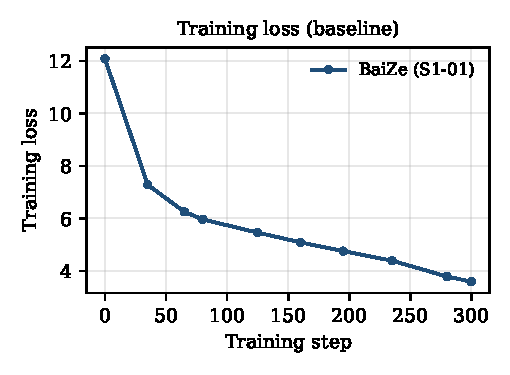
\includegraphics[width=\columnwidth]{figures/train_loss.pdf}
\caption{Training loss of the baseline (S1-01) over 300 steps. The final bend marks the exponential WSD decay phase.}
\label{fig:loss}
\end{figure}

Figure~\ref{fig:ablation} summarises the short-horizon (80-step) losses across swept configurations, visualising the two clear findings: the architecture is already optimal, and the only productive lever is the stable learning rate.

\begin{figure}[htbp]
\centering
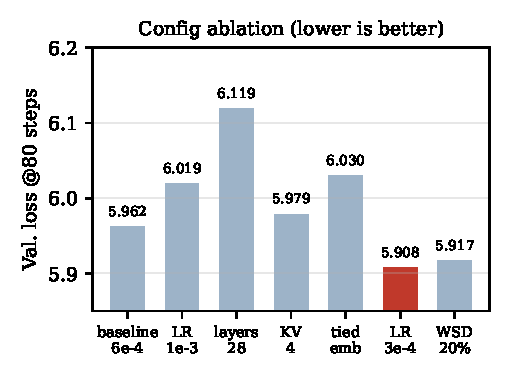
\includegraphics[width=\columnwidth]{figures/config_ablation.pdf}
\caption{Short-horizon (80-step) validation loss across swept configurations. Lower is better. The winning configuration (S3-01) is highlighted.}
\label{fig:ablation}
\end{figure}

\subsection{Architecture Selection Evidence at 2B}\label{sec:arch2b}
To anchor the architecture choice (Section~\ref{sec:arch-rationale}) in controlled experiment rather than availability alone, we trained two candidate 2B backbones---MiniCPM5-2B (dense) and Mamba2-hybrid (Nemotron-H style)~\cite{dao2024transformers,nvidia2025nemotronh}---from scratch under identical data, seed, and 6-GPU (TP1/DP6) settings for 1000 steps, then profiled inference with a shared mcore direct driver.
Table~\ref{tab:arch2b} reports the three-way comparison: the hybrid wins two of three axes---lower loss with fewer parameters, and faster inference---while the dense model retains a $\sim$24\% training-throughput edge.
This positions Mamba2-hybrid as the preferred 2B backbone for inference-heavy deployments, while the dense GQA design stays optimal for the budget-constrained 1B agent built here.
The dense model's low decode rate is a mcore direct-driver artefact (per-layer fused-attention CPU launch overhead, CPU-bound) rather than a fundamental inefficiency; both backbones share the same measurement path, so the relative decode comparison ($\times$10.3) remains trustworthy.

\begin{table}[htbp]
\centering
\caption{Matched 2B-scale dense-vs-hybrid comparison (1000 steps, seq 4096, GBS 6, TP1/DP6, BF16; inference: mcore direct driver, TP1, BF16, seq-2048 prompt + 256 gen).}
\label{tab:arch2b}
\begin{tabular}{lccc}
\toprule
\textbf{Metric} & \textbf{MiniCPM5-2B} & \textbf{Mamba2-hybrid} & \textbf{Winner} \\
\midrule
Parameters & 2.512B & \textbf{2.220B} & hybrid ($-11.6\%$) \\
Final loss (1000 steps) & 4.8065 & \textbf{4.6846} & hybrid \\
Training tok/s (6 cards) & \textbf{$\sim$89k} & $\sim$72k & dense ($+24\%$) \\
Prefill tok/s & 21{,}436 & \textbf{23{,}692} & hybrid ($+10.5\%$) \\
Decode tok/s & 2.21 & \textbf{22.77} & hybrid ($\times$10.3) \\
\bottomrule
\end{tabular}
\end{table}
\section{Conclusion}

We presented BaiZe, a 1.04B-parameter agentic language model built from scratch on a fixed $\sim$84\,GPU-hour budget.
Through a staged, budget-constrained search under $\mu$P hyper-parameter transfer and a WSD schedule, we isolated the single most productive lever---the stable-phase learning rate---and improved validation loss from $5.086$ to $4.969$ ($-0.117$) at matched step counts, with $\approx$102--111\,k tokens/s throughput on $8\times$H100.
Our architecture analysis confirmed that the Llama-style GQA baseline is well-placed in the 1B regime, where Megatron-Core offers no hybrid or Nemotron-style variant; a complementary matched 2B-scale comparison further showed that a Mamba2-hybrid backbone attains lower loss and faster inference with fewer parameters, charting the family's evolution path toward 2B while the dense design stays optimal for the budget-constrained 1B agent built here.

The complete recipe and a single reproducible command encapsulate the entire construction; the next step is agentic fine-tuning with the \texttt{UltraData-SFT-Agent} corpus toward a deployable agent core for EDA and embedded applications.
We hope this blueprint lowers the barrier for cost-bounded teams building their own efficient agentic SLMs from scratch.

\bibliographystyle{IEEEtran}
\bibliography{reference}

\end{document}